\section{Conclusions}\label{sec:concl}
% Auxiliary texts
Figure \ref{Fig:Load_timediscritized_A} plots the evolution of the total vertical reaction applied at the sample's top edge with respect to the displacement loading for different loading rates with model A. All cases show similar trends. After the crack starts to evolve, approximately at $t=\dots$, the total reaction begins to decrease significantly.

\begin{figure}[htbp]
    \centering
    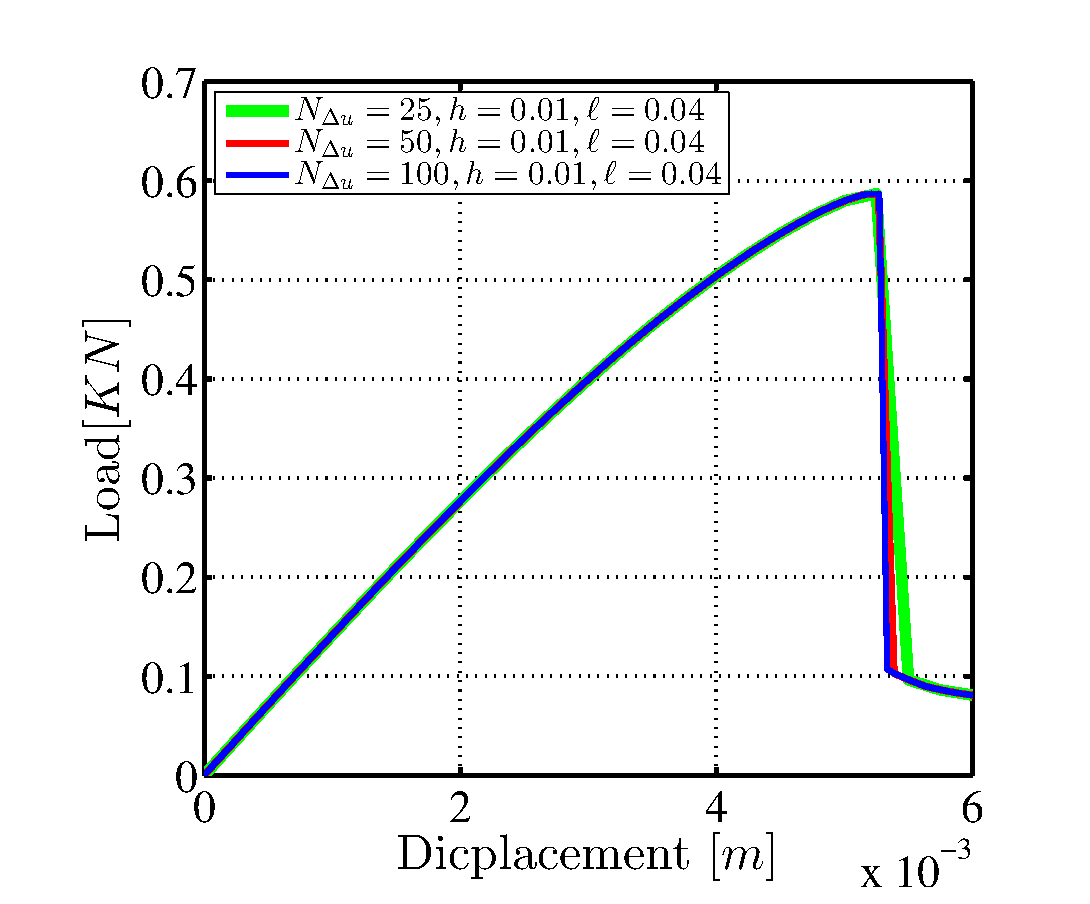
\includegraphics[width=0.8\textwidth]{Load_timediscritized.eps}
    \caption{{Cracked square plate under a tension test with different $\dot{u}_D$.} Total vertical reaction on the top edge versus time for different number of load steps. The total reaction is normalized by \dots, i.e., by the total reaction applied to the top edge at $t=t_f$ in the case without any crack or phase field evolution. {Here $t_f=\dots$s.}
    All models give rise to similar trends for the total reaction at the top. The total reaction begins to decrease at approximately $t=\dots t_f$ when the cracks start to propagate.}
    \label{Fig:Load_timediscritized_A}
\end{figure}

Figure \ref{Fig:Force_MESHSIZE_fracture_A.eps} depicts the evolution of the total vertical reaction applied at the sample's top edge with respect to the imposed displacement for different $h$ with model A.

\begin{figure}[htbp]
    \centering
    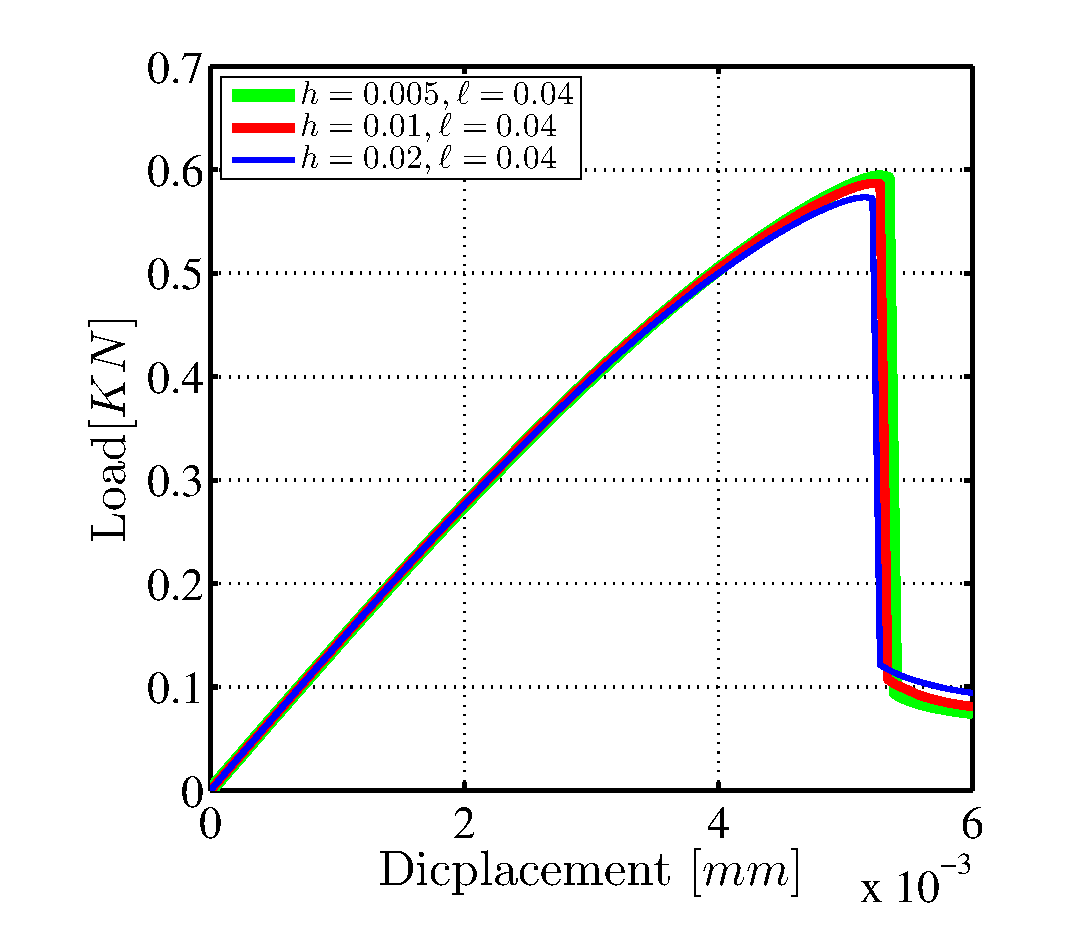
\includegraphics[width=0.8\textwidth]{FIG4_Force_MESHSIZE_fracture.eps}
    \caption{{Cracked square plate under a tension test with different $h$.} Total vertical reaction on the top edge versus time for different mesh size $h$. The total reaction is normalized by \dots, i.e., by the total reaction applied to the top edge at $t=t_f$ in the case without any crack or phase field evolution. {Here $t_f=\dots$s.}
    All models give rise to similar trends for the total reaction at the top. The total reaction begins to decrease at approximately $t=\dots t_f$ when the cracks start to propagate.}
    \label{Fig:Force_MESHSIZE_fracture_A.eps}
\end{figure}

Figure \ref{Fig:Force_Ell_fracture_A.eps} plots the same output as Figure \ref{Fig:Force_MESHSIZE_fracture_A.eps} with different $\ell$, while we keep other parameters similar for all tests.
\begin{figure}[htbp]
    \centering
    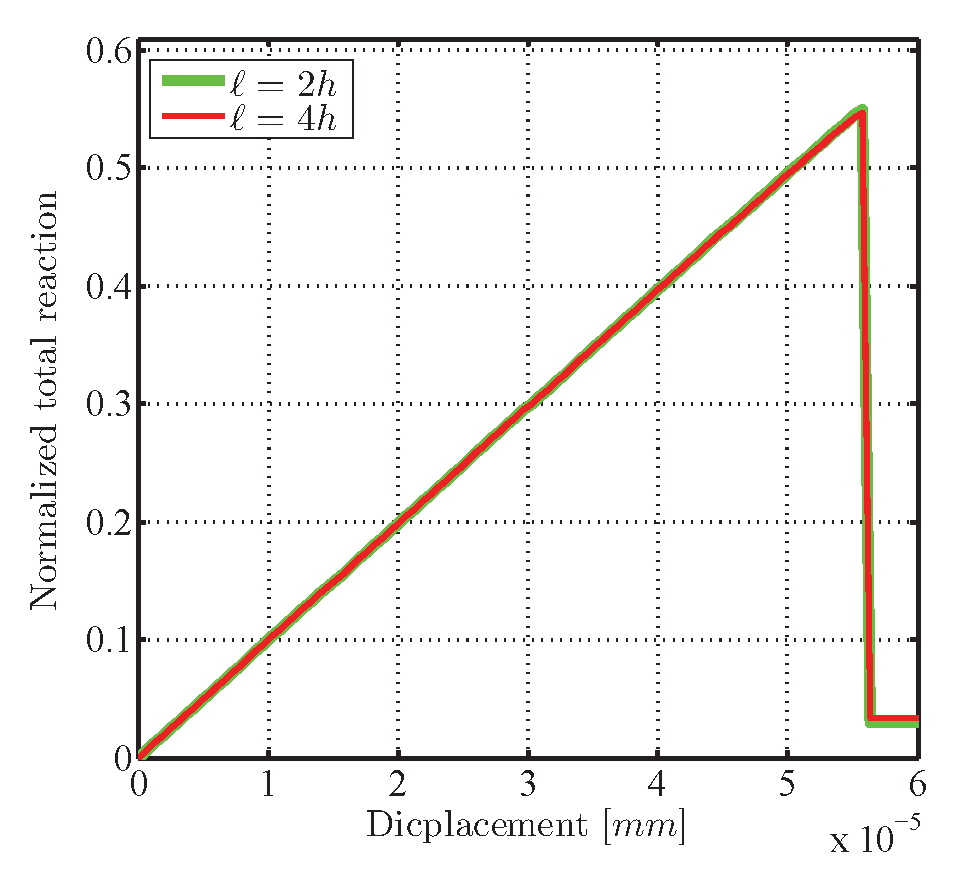
\includegraphics[width=0.8\textwidth]{Force_ELL_fracture.eps}
    \caption{{Cracked square plate under a tension test with different $h$.} Total vertical reaction on the top edge versus time for different regularization parameter $\ell$. The total reaction is normalized by \dots, i.e., by the total reaction applied to the top edge at $t=t_f$ in the case without any crack or phase field evolution. {Here $t_f=\dots$s.}
    All models give rise to similar trends for the total reaction at the top. The total reaction begins to decrease at approximately $t=\dots t_f$ when the cracks start to propagate.}
    \label{Fig:Force_Ell_fracture_A.eps}
\end{figure}















